% 建议使用 XeLaTeX 或 LuaLaTeX 编译(更佳的中文支持)
\documentclass[UTF8,zihao=-4]{ctexart}

% 统一导言
\usepackage[a4paper,margin=2.5cm]{geometry}
\usepackage{amsmath,amssymb,amsthm}
\usepackage{bm}
\usepackage{hyperref}
\usepackage{graphicx}
\usepackage{caption}
\usepackage{listings}
\usepackage{xcolor}
\usepackage{float}
\usepackage{placeins}

% 图片路径
\graphicspath{{figures/}}

% 统一代码风格
\lstdefinestyle{code}{%
  language=Python,
  basicstyle=\ttfamily\small,
  numbers=left,
  numberstyle=\tiny,
  keywordstyle=\color{blue}\bfseries,
  commentstyle=\color{teal!70!black},
  stringstyle=\color{orange!70!black},
  breaklines=true,
  frame=single,
  rulecolor=\color{black!30},
  tabsize=2,
  showstringspaces=false
}
\lstset{style=code}

\title{k-近邻(k-NN):理论与实践}
\author{}
\date{\today}

\begin{document}
\maketitle

% 结构:Introduction / Theory and Formulas / Applications and Tips / Python Practice / Result / Summary

\section{引言}
k-近邻(k-Nearest Neighbors, k-NN)是一种非参数、基于实例的“惰性学习”方法:预测时在训练集中查找与查询样本最近的 $k$ 个邻居。其思想直观、实现简单,在低维、良好缩放的数据上常有竞争力,但对特征缩放敏感,并在高维下性能下降。

\section{原理与公式}
给定查询点 $\mathbf{x}$,在指定距离度量 $d(\cdot,\cdot)$(如欧氏、曼哈顿)下找到其最近的 $k$ 个邻居。分类任务采用多数表决(可选距离加权 \texttt{weights=distance} 使近邻权重更高);回归任务取邻居目标值的平均(或距离加权平均)。

计算上,朴素查找每次预测代价为 $\mathcal{O}(nd)$($n$ 为样本数,$d$ 为维度)。中等维度时可使用 KDTree/BallTree 提速。k-NN 受“维度灾难”影响,合适的特征缩放与度量选择至关重要。

\section{应用与技巧}
\begin{itemize}
  \item \textbf{选择 k:} 通过交叉验证调参;二分类常取奇数 $k$ 以减少平票。
  \item \textbf{缩放:} 对特征做标准化/归一化,或使用 Pipeline;距离对量纲非常敏感。
  \item \textbf{度量:} 尝试欧氏与曼哈顿;必要时考虑领域特定距离。
  \item \textbf{权重:} \texttt{uniform} 与 \texttt{distance} 可对类间重叠区产生不同效果。
  \item \textbf{复杂度:} 预测代价随数据量增长;大规模可考虑近似近邻检索。
\end{itemize}

\section{Python 实战}
在本章节目录运行下述命令,图片将保存到 \texttt{figures/}:
\begin{lstlisting}[style=code,caption={生成 k-NN 配图},label={lst:genfigs_knn_cn}]
python gen_knn_figures.py
\end{lstlisting}

% 纳入完整 Python 源码
\lstinputlisting[style=code,caption={gen\_knn\_figures.py 源码},label={lst:source_knn_cn}]{gen_knn_figures.py}

\section{结果}
\begin{figure}[H]
  \centering
  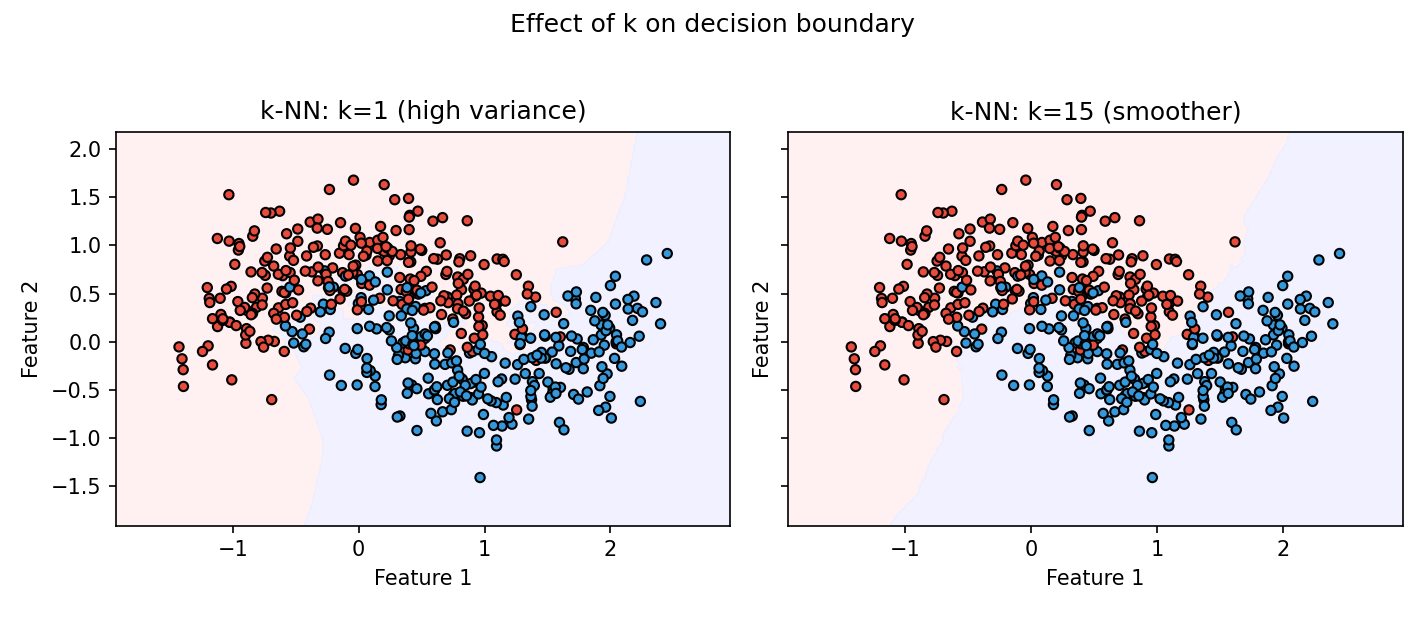
\includegraphics[width=0.95\linewidth]{knn_k_compare.png}
  \caption{不同 k(1 vs 15)的决策边界对比。}
  \label{fig:knn_k_cn}
\end{figure}
\FloatBarrier

\begin{figure}[H]
  \centering
  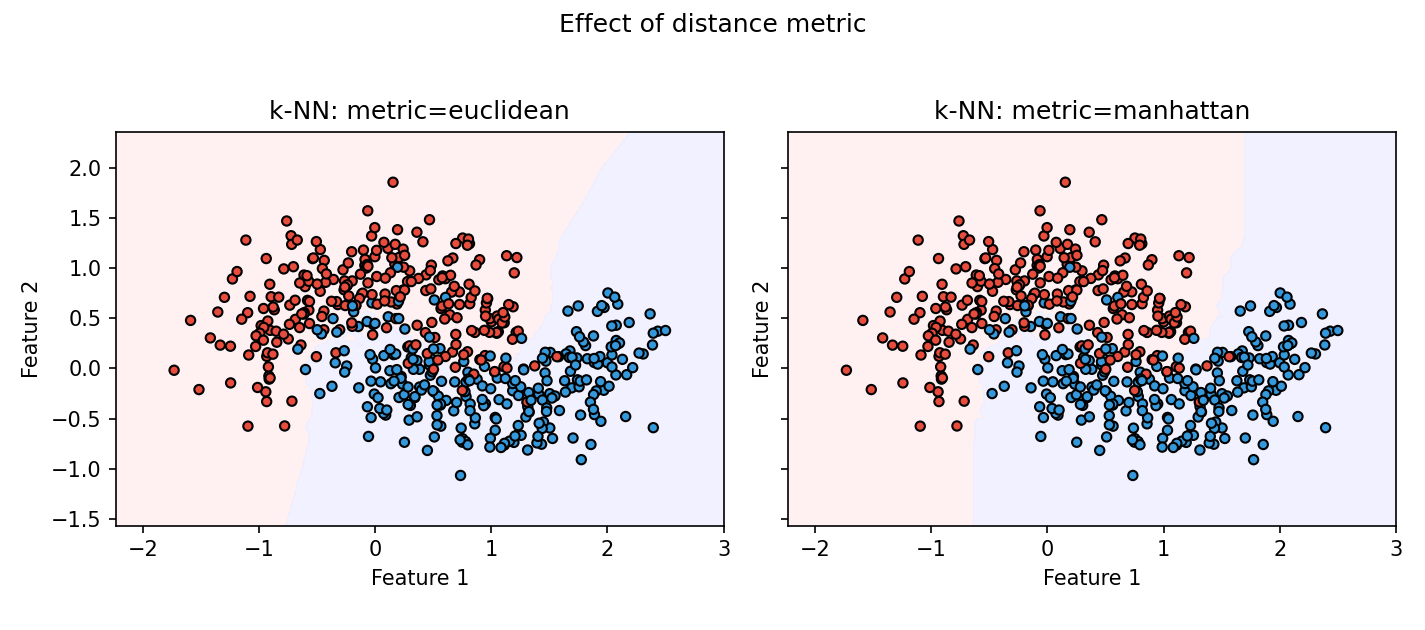
\includegraphics[width=0.95\linewidth]{knn_metric_compare.png}
  \caption{不同距离度量:欧氏(Euclidean) vs 曼哈顿(Manhattan)。}
  \label{fig:knn_metric_cn}
\end{figure}
\FloatBarrier

\begin{figure}[H]
  \centering
  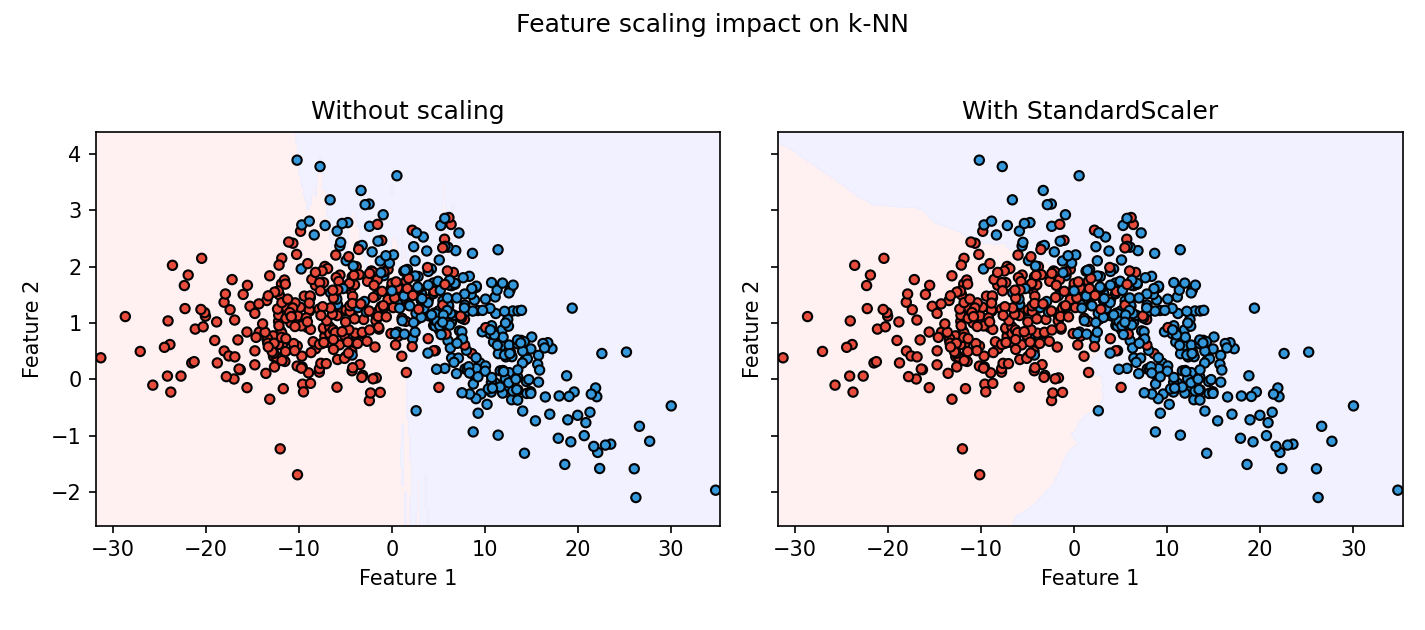
\includegraphics[width=0.95\linewidth]{knn_scaling_effect.png}
  \caption{特征缩放对决策边界的影响。}
  \label{fig:knn_scale_cn}
\end{figure}
\FloatBarrier

\begin{figure}[H]
  \centering
  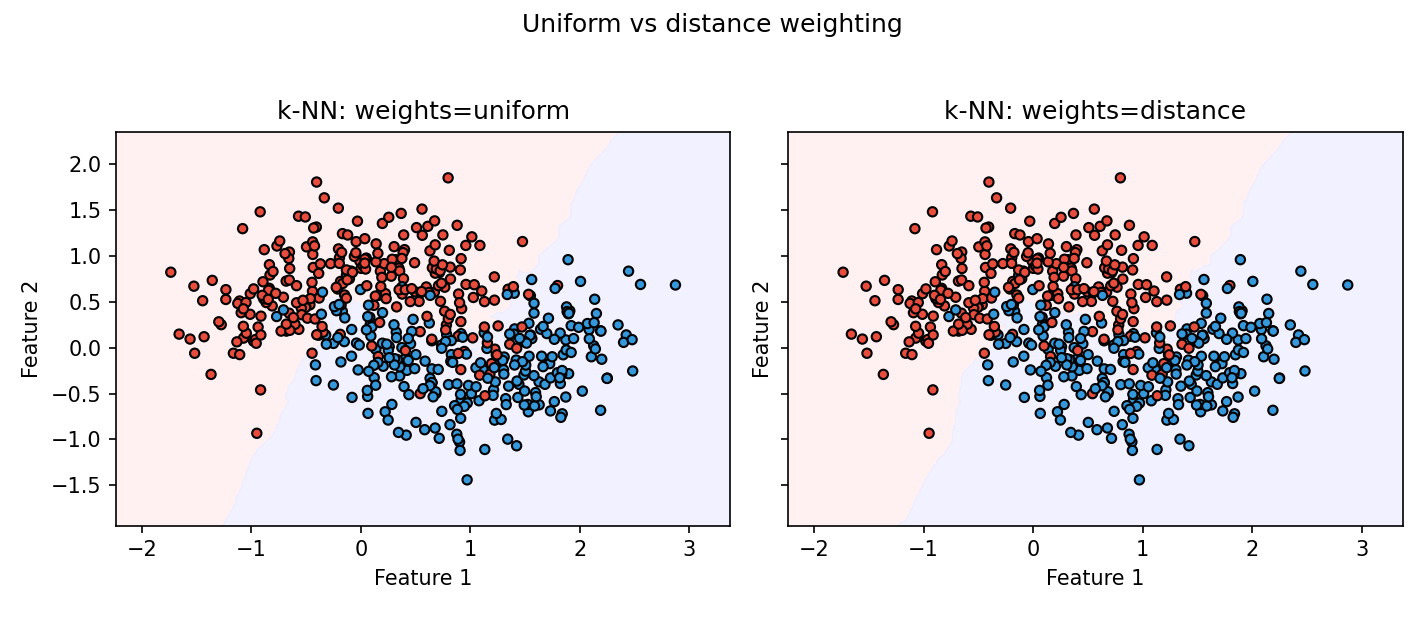
\includegraphics[width=0.95\linewidth]{knn_weight_compare.png}
  \caption{均匀权重 vs 距离加权的对比。}
  \label{fig:knn_weight_cn}
\end{figure}
\FloatBarrier

\begin{figure}[H]
  \centering
  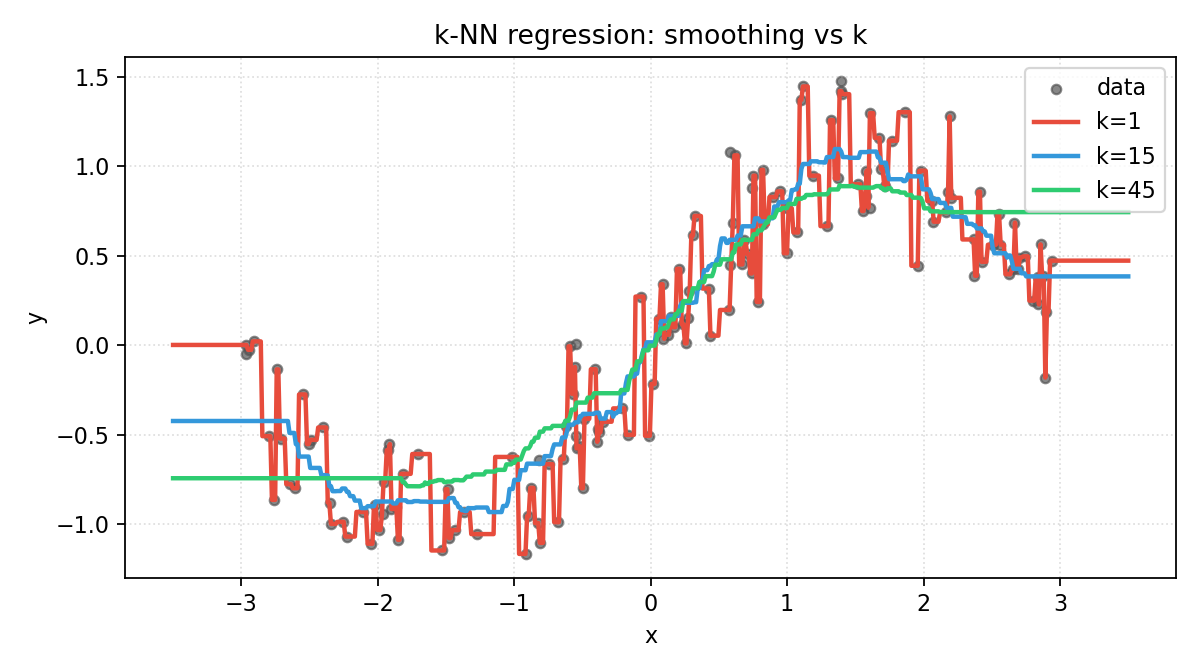
\includegraphics[width=0.85\linewidth]{knn_regression_curve.png}
  \caption{k-NN 回归:随 k 增大平滑程度的变化。}
  \label{fig:knn_reg_cn}
\end{figure}
\FloatBarrier

\section{总结}
k-NN 在特征良好缩放且维度适中的场景下是简洁有效的基线。通过验证选择合适的 $k$、距离度量与权重设置,并做好缩放预处理,可获得稳定表现。

\end{document}

